\documentclass[xcolor = {dvipsnames, table}]{beamer}

\definecolor{dotlightblue} {HTML}{ADD8E6}
\definecolor{dotlightcoral}{HTML}{F08080}

\RequirePackage[english]{babel}
\RequirePackage[utf8]{inputenc}

\RequirePackage{fancyvrb}

\RequirePackage{listings}
\lstset{
    language = C,
    basicstyle = \ttfamily,
}

% \set{}
\RequirePackage{braket}

\RequirePackage{amsmath}

\RequirePackage{tikz}
% for arrows inside listings
\usetikzlibrary{decorations.text, calc}
\usetikzlibrary{positioning, matrix, arrows.meta}
\newcommand{\tikzmark}[2]{%
     \tikz[overlay,remember picture]%
        \node[text=black, inner sep=2pt] (#1) {#2};%
}

\RequirePackage{algorithm}
\RequirePackage[noend]{algpseudocode}

\algnewcommand \algorithmicin{\textbf{in}}
\algnewcommand \In {\algorithmicin\ }
\algnewcommand \algorithmiccontinue{\textbf{continue}}
\algnewcommand \Continue {\State \algorithmiccontinue\ }
\algnewcommand \algorithmicskip{\textbf{skip}}
\algnewcommand \Skip {\State \algorithmicskip\ }
\algrenewtext{ForAll}[2]%
    {\algorithmicfor\ #1 \algorithmicin\ #2 \algorithmicdo}
\algnewcommand \SkipIf[1] {\State \algorithmicskip\ \algorithmicif\ #1}

% reduce the size of the font in algorithms slightly
\makeatletter
\renewcommand{\ALG@beginalgorithmic}{\footnotesize}
\makeatother

\AtBeginSection[]{
    \begin{frame}
        \vfill
        \centering
        \begin{beamercolorbox}[sep=8pt,center,shadow=true,rounded=true]{title}
            \usebeamerfont{title}\insertsectionhead\par%
        \end{beamercolorbox}
        \vfill
    \end{frame}
}

% https://tex.stackexchange.com/questions/142672/uncovering-lines-in-an-equation-in-split-environment
\newcommand{\disponslide}[2]{%
    \alt<#1>{#2}{\phantom{#2}}
}

%Information to be included in the title page:
\title{Theory makes beautiful programs}
\author{Jørgen Kvalsvik j@lambda.is}
\date{31/08/2022}

\begin{document}
\frame{\titlepage}

\begin{frame}
    \begin{block}{Topics}
        \item Brief introduction to MC/DC
        \item A (thorough) description of the algorithm in gcc (notation
            warning)
        \item Some ramblings on thinking before typing
    \end{block}
\end{frame}

\begin{frame}
    Modified condition/decision coverage (MC/DC)

    \begin{itemize}
        \item Why care about coverage?
        \item How is it different from branch coverage?
        \item What does maths have to do with it?
    \end{itemize}
\end{frame}

\begin{frame}
    Why even care?
    \begin{columns}
        \begin{column}{0.5\textwidth}
            \includegraphics[width = \textwidth]{img/bureaucrat.png}
        \end{column}

        \begin{column}{0.5\textwidth}
            \begin{itemize}
                \item DO-178B/C (Level A)
                \item ISO26262 (ASIL D)
            \end{itemize}
        \end{column}
    \end{columns}
\end{frame}

\newcommand \rowhl {\rowcolor{Cyan!20}}

\begin{frame}[fragile]
    The problem with branch coverage
    \begin{columns}
        \begin{column}{0.5\textwidth}
            \begin{lstlisting}
if ((a && b) || c) {
    //
} else {
    //
}
            \end{lstlisting}
        \end{column}

        \begin{column}{0.5\textwidth}
            \begin{tabular}{c c c c}
                        a & b & c \\
                        \hline
                \rowhl  F & F & F & F \\
                \rowhl  F & F & T & T \\
                        F & T & F & F \\
                        F & T & T & T \\
                        T & F & F & F \\
                        T & F & T & T \\
                        T & T & F & T \\
                        T & T & T & T \\
            \end{tabular}
        \end{column}
    \end{columns}
\end{frame}

\begin{frame}
    Modified condition/decision coverage satisfied if:
    \begin{itemize}
        \item every entry and exit point has been invoked
        \item every basic condition has taken on all possible outcomes
        \item each basic condition has been shown to independently affect the
              decision’s outcome
    \end{itemize}
\end{frame}

\begin{frame}[fragile]
    \begin{columns}
        \begin{column}{0.7\textwidth}
            \begin{lstlisting}[basicstyle = \footnotesize\ttfamily]
if ((a && b) || c) {
    //
} else {
    //
}
            \end{lstlisting}

            \begin{itemize}
                \item every entry and exit point has been invoked
            \end{itemize}

            Branch coverage (or decision coverage)
        \end{column}

        \begin{column}{0.3\textwidth}
            \begin{tabular}{c c c c}
                        a & b & c \\
                        \hline
                \rowhl  F & F & F & F \\
                \rowhl  F & F & T & T \\
                        F & T & F & F \\
                        F & T & T & T \\
                        T & F & F & F \\
                        T & F & T & T \\
                        T & T & F & T \\
                        T & T & T & T \\
            \end{tabular}
        \end{column}
    \end{columns}
\end{frame}

\begin{frame}[fragile]
    \begin{columns}
        \begin{column}{0.7\textwidth}
            \begin{lstlisting}[basicstyle = \footnotesize\ttfamily]
if ((a && b) || c) {
    //
} else {
    //
}
            \end{lstlisting}
            \begin{itemize}
                \item every basic condition has taken on all possible outcomes
            \end{itemize}

            Condition coverage
        \end{column}

        \begin{column}{0.3\textwidth}
            \begin{tabular}{c c c c}
                        a & b & c \\
                        \hline
                \rowhl  F & F & F & F \\
                        F & F & T & T \\
                        F & T & F & F \\
                        F & T & T & T \\
                        T & F & F & F \\
                \rowhl  T & F & T & T \\
                \rowhl  T & T & F & T \\
                        T & T & T & T \\
            \end{tabular}
        \end{column}
    \end{columns}
\end{frame}

\begin{frame}[fragile]
    \begin{columns}
        \begin{column}{0.7\textwidth}
            \begin{lstlisting}[basicstyle = \footnotesize\ttfamily]
if ((a && b) || c) {
    //
} else {
    //
}
            \end{lstlisting}
            \begin{itemize}
                \item each basic condition has been shown to
                      \emph{independently} affect the decision’s outcome
            \end{itemize}
            Modified condition/decision coverage
        \end{column}

        \begin{column}{0.3\textwidth}
            \begin{tabular}{c c c c}
                        a & b & c \\
                        \hline
                \rowhl  F & F & F & F \\
                \rowhl  F & F & T & T \\
                        F & T & F & F \\
                        F & T & T & T \\
                \rowhl  T & F & F & F \\
                        T & F & T & T \\
                \rowhl  T & T & F & T \\
                        T & T & T & T \\
            \end{tabular}
        \end{column}
    \end{columns}
\end{frame}

\begin{frame}
    \begin{itemize}
        \item Testing all $2^N$ inputs would not give more information
        \item Requires $N+1$ test cases
        \item Can catch bad logic
    \end{itemize}
\end{frame}

\begin{frame}
    The problem with MC/DC

    \begin{itemize}
        \item Only tests implementation, not the spec
        \item Possible to cheat
        \item Needs many test cases in maybe uninteresting places
        \item \emph{Awful} without tooling
    \end{itemize}
\end{frame}

\begin{frame}[fragile]
    I wrote a patch for gcc

    \begin{block}{}
        \begin{Verbatim}[fontsize = \footnotesize]
$ git log -n 1 --format=short --shortstat
Author: Jørgen Kvalsvik <jorgen.kvalsvik@woven-planet.global>

    Add condition coverage profiling

21 files changed, 2952 insertions(+), 27 deletions(-)
        \end{Verbatim}
    \end{block}

    \begin{block}{}
        \begin{Verbatim}[fontsize=\footnotesize]
 gcc/tree-profile.cc |  +978
        \end{Verbatim}
    \end{block}
\end{frame}

\begin{frame}[fragile]
    \begin{block}{Demo}
        \begin{lstlisting}[language = sh, basicstyle = \scriptsize\ttfamily]
$ gcc --coverage -fprofile-conditions
    demo.c -o demo
$ ./demo 0 0 0
$ ./demo 0 0 1
$ ./demo 1 0 0
$ gcov --conditions demo
$ cat demo.c.gcov

    if ((a && b) || c) {
condition outcomes covered 4/6
condition  0 not covered (true)
condition  1 not covered (true)
        \end{lstlisting}
    \end{block}

    \begin{block}{Question}
        Why is \lstinline{a = 1} not covered?
    \end{block}
\end{frame}

\begin{frame}
    \begin{itemize}
        \item each basic condition has been shown to \emph{independently}
              affect the decision’s outcome
    \end{itemize}

    \begin{block}{Definition}
        A condition independently affects the outcome if changing it while
        keeping the other values constant changes the outcome
    \end{block}
\end{frame}

\begin{frame}[fragile]
    \begin{columns}
        \begin{column}{0.5\textwidth}
            \begin{lstlisting}[basicstyle = \footnotesize\ttfamily]
    if ((a && b) || c) {
        //
    } else {
        //
    }
            \end{lstlisting}
        \end{column}

        \begin{column}{0.5\textwidth}
            \begin{tabular}{c c c c}
                        a & b & c \\
                        \hline
                 \rowhl F & F & F & F \\
                        F & F & T & T \\
                        F & T & F & F \\
                        F & T & T & T \\
                \rowhl  T & F & F & F \\
                        T & F & T & T \\
                        T & T & F & T \\
                        T & T & T & T \\
            \end{tabular}
        \end{column}
    \end{columns}

    \begin{block}{Observation}
        Changing \lstinline{a} does not change the decision
    \end{block}
\end{frame}

\begin{frame}
    This effect is called \emph{masking}

    \begin{itemize}
        \item \lstinline{* || true}
        \item \lstinline{* && false}
    \end{itemize}
\end{frame}

\begin{frame}
    \begin{block}{Commutation}
        Reversing a boolean expression does not change its truth table
        \begin{align*}
            (P \wedge Q) & \equiv (Q \wedge P) \\
            (P \vee Q)   & \equiv (Q \vee P)   \\
        \end{align*}
    \end{block}

    \begin{block}{Observation}
        Masked conditions are \emph{short circuited} in the reversed expression
    \end{block}
\end{frame}

\begin{frame}
    \centering
    \begin{columns}
        \begin{column}{0.3\textwidth}
            \centering
            \lstinline{(a && b) || c}
            \begin{tabular}{c c c c}
                a & b & c & \\
                \hline
                F & * & F & F \\
                F & * & T & T \\
                F & * & F & F \\
                F & * & T & T \\

                T & F & F & F \\
                T & F & T & T \\
                T & T & * & T \\
                T & T & * & T \\
            \end{tabular}
        \end{column}

        \begin{column}{0.3\textwidth}
            \centering
            \lstinline{c || (b && a)}
            \begin{tabular}{c c c c}
                c & b & a & \\
                \hline
                F & F & - & F \\
                F & F & - & F \\
                F & T & F & F \\
                F & T & T & T \\

                T & - & - & T \\
                T & - & - & T \\
                T & - & - & T \\
                T & - & - & T \\
            \end{tabular}
        \end{column}
    \end{columns}
\end{frame}

\begin{frame}
    \begin{columns}
        \begin{column}{0.3\textwidth}
            \centering
            \lstinline{(a && b) || c}
            \begin{tabular}{c c c c}
                a & b & c & \\
                \hline
                F & * & F & F \\
                F & * & T & T \\
                F & * & F & F \\
                F & * & T & T \\

                T & F & F & F \\
                T & F & T & T \\
                T & T & * & T \\
                T & T & * & T \\
            \end{tabular}
        \end{column}

        \begin{column}{0.3\textwidth}
            \centering
            \lstinline{c || (b && a)}
            \begin{tabular}{c c c c}
                c & b & a & \\
                \hline
                F & F & - & F \\
                T & - & - & T \\
                F & T & F & F \\
                T & - & - & T \\

                F & F & - & F \\
                T & - & - & T \\
                F & T & T & T \\
                T & - & - & T \\
            \end{tabular}
        \end{column}

        \begin{column}{0.3\textwidth}
            \centering
            \lstinline{(a && b) || c}
            \begin{tabular}{c c c c}
                a & b & c & \\
                \hline
                F & * & F & F \\
                - & - & T & T \\
                F & * & F & F \\
                - & - & T & T \\

                T & F & F & F \\
                - & - & T & T \\
                T & T & * & T \\
                T & T & * & T \\
            \end{tabular}
        \end{column}
    \end{columns}

    \begin{block}{Note}
        Row order in \lstinline{c || (b && a)} changed
    \end{block}
\end{frame}

\begin{frame}
    \centering\lstinline{(a && b) || c}
    \begin{columns}
        \begin{column}{0.3\textwidth}
            \centering
            \begin{tabular}{c c c c}
                        a & b & c & \\
                        \hline
                \rowhl  F & * & F & F \\
                \rowhl  - & - & T & T \\
                        F & * & F & F \\
                        - & - & T & T \\

                \rowhl  T & F & F & F \\
                        - & - & T & T \\
                \rowhl  T & T & * & T \\
                        T & T & * & T \\
            \end{tabular}
        \end{column}

        \begin{column}{0.3\textwidth}
            \centering
            \begin{tabular}{c c c c}
                        a & b & c \\
                        \hline
                \rowhl  F & F & F & F \\
                \rowhl  F & F & T & T \\
                        F & T & F & F \\
                        F & T & T & T \\
                \rowhl  T & F & F & F \\
                        T & F & T & T \\
                \rowhl  T & T & F & T \\
                        T & T & T & T \\
            \end{tabular}
        \end{column}
    \end{columns}
\end{frame}

\begin{frame}
    \begin{block}{Bad logic}
        \begin{tabular}{l l}
            Specification  & \texttt{(a \&\& b)\quad || c} \\
            Implementation & \texttt{(a \&\& !c) || c} \\
        \end{tabular}
    \end{block}
\end{frame}

\begin{frame}[fragile]
    \begin{columns}
        \begin{column}{0.3\textwidth}
            \centering
            Masking table
            \begin{tabular}{c c c c}
                        a & b & c & \\
                        \hline
                        F & * & F & F \\
                        - & - & T & T \\
                        F & * & F & F \\
                        - & - & T & T \\

                        T & F & F & F \\
                        - & - & T & T \\
                        T & T & * & T \\
                        T & T & * & T \\
            \end{tabular}
        \end{column}

        \begin{column}{0.3\textwidth}
            \centering
            \lstinline{(a && !c) || c}
            \begin{tabular}{c c c c}
                        a & !c & c & \\
                        \hline
                        F & * & F & F \\
                        - & - & T & T \\
                        F & * & F & F \\
                        - & - & T & T \\

                        T & T & * & T \\
                        - & - & T & T \\
                        T & T & * & T \\
                        T & T & * & T \\
            \end{tabular}
        \end{column}
    \end{columns}
\end{frame}

\begin{frame}[fragile]
    Cheating MC/DC
    \begin{columns}
        \begin{column}{0.4\textwidth}
            \centering
            \begin{lstlisting}[basicstyle = \footnotesize\ttfamily]
if ((a && b) || c) {
    //
} else {
    //
}
            \end{lstlisting}

        \end{column}

        \begin{column}{0.4\textwidth}
            \centering
            \begin{lstlisting}[basicstyle = \footnotesize\ttfamily]
int ab = a && b;
if (ab || c) {
    //
} else {
    //
}
            \end{lstlisting}
        \end{column}
    \end{columns}

    \begin{columns}
        \begin{column}{0.4\textwidth}
            \centering
            \begin{tabular}{c c c c}
                        a & b & c \\
                        \hline
                \rowhl  F & F & F & F \\
                \rowhl  F & F & T & T \\
                        F & T & F & F \\
                        F & T & T & T \\
                \rowhl  T & F & F & F \\
                        T & F & T & T \\
                \rowhl  T & T & F & T \\
                        T & T & T & T \\
            \end{tabular}
        \end{column}

        \begin{column}{0.4\textwidth}
            \centering
            \begin{tabular}{c c}
                        ab & c \\
                        \hline
                 \rowhl F & F \\
                        F & T \\
                 \rowhl T & F \\
                 \rowhl T & T \\
            \end{tabular}
        \end{column}
    \end{columns}
\end{frame}

\begin{frame}
    \begin{block}{Writing beautiful programs}
        \begin{itemize}
            \item Start solving for simple examples - a general solution
                \emph{also} solves simple inputs, draw insights from these
            \item For every added (failing) case, understand \emph{why} it failed
            \item Theory-based programs almost self-materialize, easy to write
            \item Regular Expression Matching Can Be Simple And Fast (Russ Cox)
            \item In gcc: a bunch of (mostly) simple relationships put together
        \end{itemize}
    \end{block}
\end{frame}

\section{Control flow graphs}

\begin{frame}[fragile]
    \begin{columns}
        \begin{column}{0.4\textwidth}
            \begin{lstlisting}[basicstyle = \footnotesize\ttfamily]
if ((a && b) || c) {
    // t
} else {
    // f
}
// e
            \end{lstlisting}
        \end{column}
        \begin{column}{0.4\textwidth}
            \begin{lstlisting}[basicstyle = \footnotesize\ttfamily]
_a:
  if (a) goto _b
  else   goto _c
_b:
  if (b) goto _t
  else   goto _c
_c:
  if (c) goto _t
  else   goto _f
_t:
  goto _e
_f:
  goto _e
_e:
            \end{lstlisting}
        \end{column}
    \end{columns}
\end{frame}

\begin{frame}[fragile]
    \begin{columns}
        \begin{column}{0.4\textwidth}
            \begin{lstlisting}[basicstyle = \footnotesize\ttfamily]
if ((a && b) || c) {
    // t
} else {
    // f
}
// e
            \end{lstlisting}
        \end{column}
        \begin{column}{0.4\textwidth}
            \includegraphics[width = \linewidth, keepaspectratio]{graph/fig1.pdf}
        \end{column}
    \end{columns}
\end{frame}

\begin{frame}
    \begin{block}{Control flow graph}
        \begin{itemize}
            \item Directed graph
            \item Nodes are an uninterruptible sequence of instructions
            \item Edges are next possible paths of execution
            \item Edges are labelled fallthrough, true/false (conditional), complex
            \item Fallthrough and conditional are mutually exclusive
        \end{itemize}
    \end{block}
\end{frame}

\section{Act I: Inferring decisions}
\begin{frame}[fragile]
    \begin{columns}
        \begin{column}{0.4\textwidth}
            \begin{lstlisting}[basicstyle = \footnotesize\ttfamily]
if ((a && b) || c) {
    // t
} else {
    // f
}
// e
            \end{lstlisting}
        \end{column}
        \begin{column}{0.4\textwidth}
            \includegraphics[width = \linewidth, keepaspectratio]{graph/fig2.pdf}
        \end{column}
    \end{columns}
\end{frame}

\begin{frame}
    \begin{equation*}
        \bigcup \set{Succ(v) \mid v \in B} = N[B]
    \end{equation*}
    \begin{equation*}
        N[B] = B \cup O_B
    \end{equation*}

    \begin{tabular}{l l}
        $B$    & is a decision (boolean expression) \\
        $O_B$  & is the \emph{outcome} of $B$ \\
        $N(B)$ & is the \emph{open neighborhood} of $B$ \\
        $N[B]$ & is the \emph{closed neighborhood} of $B$ \\
    \end{tabular}
\end{frame}

\begin{frame}[fragile]
    \begin{columns}
        \begin{column}{0.5\textwidth}
            \begin{lstlisting}[escapeinside={*@}{@*}, aboveskip = 5em]
if (*@\tikzmark{fst}{}@*(a && b) || c*@\tikzmark{lst}{}@*) {
*@\tikzmark{then}{}@*
} else {
*@\tikzmark{else}{}@*
}
            \end{lstlisting}

            \begin{tikzpicture}[overlay,remember picture]
                \node (fst) at ($(fst) + (0.0em, +1.75ex)$) {};
                \node (lst) at ($(lst) + (0.0em, +1.75ex)$) {};
                \node (top) at ([yshift = 3em]$(fst)!0.5!(lst)$)
                        {uninterruptible};
                \draw [->] (top) to (fst);
                \draw [->] (top) to (lst);

                \node (then) at ($(then) + (5.0em, 0.0em)$) {};
                \node (else) at ($(else) + (5.0em, 0.0em)$) {};
                \node (out) at ($(then)!0.5!(else) + (5.0em, 0.0em)$) {outcome};

                \draw [->] (out) to (then);
                \draw [->] (out) to (else);
            \end{tikzpicture}

            \only<1>{
                \begin{equation*}
                    \bigcup \set{Succ(v) \mid v \in B}
                \end{equation*}
            }

            \only<2>{
                \begin{equation*}
                    E(B) = \set{(u, v) \in E | u \in B, v \in N[B]}
                \end{equation*}
                All edges in $E(B)$ are conditional
            }

            \only<3>{
                \begin{equation*}
                    Succ(B_\Omega) = O_B
                \end{equation*}
            }

            \only<4>{
                Can not goto the middle of an \emph{expression}

                \begin{tikzpicture}[overlay,remember picture]
                    \node (nogoto) at ($(else) + (0.0em, -2.0em)$) {no goto};
                    \draw [->] (nogoto) to ($(fst)!0.5!(lst) + (0.0em, -2.0em)$);
                \end{tikzpicture}
            }
        \end{column}

        \begin{column}{0.4\textwidth}
            \only<1-2>{
                \includegraphics[
                    width  = \linewidth,
                    height = 0.8\textheight,
                    keepaspectratio,
                ]{graph/fig3.pdf}
            }
            \only<3->{
                \includegraphics[
                    width  = \linewidth,
                    height = 0.8\textheight,
                    keepaspectratio,
                ]{graph/fig4.pdf}
            }
        \end{column}
    \end{columns}
\end{frame}

\newcommand{\includegraph}[2]{%
    \includegraphics<#1>[
        width  = \linewidth,
        height = \textheight,
        keepaspectratio,
    ]{graph/#2.pdf}
}

\begin{frame}
    Reachable-by-condition-edge (BFS)
\end{frame}

\begin{frame}[fragile]
    \begin{columns}
        \begin{column}{0.4\textwidth}
            \begin{lstlisting}[basicstyle = \footnotesize\ttfamily]
if ((a && b) || c) {
    // t
} else {
    // f
}
            \end{lstlisting}
        \end{column}

        \begin{column}{0.4\textwidth}
            \includegraph{1}{fig5-1}
            \includegraph{2}{fig5-2}
            \includegraph{3}{fig5-3}
            \includegraph{4}{fig5-4}
            \includegraph{5}{fig5-5}
            \includegraph{6}{fig5-6}
            \includegraph{7}{fig5-7}
            \includegraph{8}{fig5-8}
            \includegraph{9}{fig5-9}
            \includegraph{10}{fig5-10}
            \includegraph{11}{fig5-11}
        \end{column}
    \end{columns}
\end{frame}

\begin{frame}
    \begin{algorithmic}[1]
        \Function{reach}{$v_0, v_p$}
            \State $R \gets \set{}$
            \State $Q \gets$ \Call {queue}{$v_0$}

            \Repeat
                \State $v \gets$ \Call {pop}{$Q$}
                \ForAll {$s$}{$Succs(v)$}
                    \SkipIf {$s \in R$}
                    \SkipIf {\Call {is-same}{$s, v_p$}}
                    \SkipIf {\Call {is-back-edge}{$v, s$}}
                    \SkipIf {$\neg$ \Call {dominated-by}{$s, v_0$}}
                    \SkipIf {$\neg$ \Call {is-conditional}{$s$}}
                    \State \Call {enqueue} {Q, $s$}
                    \State \Call {add}{$R, s$}
                \EndFor
            \Until{\Call {empty}{$Q$}}
            \State \Return $R$
        \EndFunction
    \end{algorithmic}
\end{frame}

\begin{frame}[fragile]
    \begin{columns}
        \begin{column}{0.4\textwidth}
            \begin{lstlisting}[basicstyle = \footnotesize\ttfamily]
if (a && b) {
    if (c) {
        // p
    } else {
        // q
    }
} else {
    // r
}
            \end{lstlisting}
        \end{column}

        \begin{column}{0.5\textwidth}
            \includegraph{1}{fig6-1}
            \includegraph{2}{fig6-2}
            \includegraph{3}{fig6-3}
            \includegraph{4}{fig6-4}
            \includegraph{5}{fig6-5}
        \end{column}
    \end{columns}
\end{frame}

\begin{frame}[fragile]
    \begin{columns}
        \begin{column}{0.6\textwidth}
            \begin{lstlisting}[basicstyle = \footnotesize\ttfamily]
if (a && b) {
    if (c) {
        // p
    } else {
        // q
    }
} else {
    // r
}
            \end{lstlisting}
            \begin{equation*}
                C = (\textcolor{dotlightblue}{G}, \textcolor{dotlightcoral}{G'})
            \end{equation*}
            \begin{equation*}
                \begin{split}
                    \forall_e \in E(G) & \bullet cond(e) \\
                    \Rightarrow & O_B \subset N[G] \\
                    \Rightarrow & B \subseteq G
                \end{split}
            \end{equation*}
        \end{column}

        \begin{column}{0.4\textwidth}
            \includegraphics[
                width   = \linewidth,
                height  = \textheight,
                keepaspectratio,
            ]{graph/fig7.pdf}
        \end{column}
    \end{columns}
\end{frame}

\begin{frame}[fragile]
    \begin{columns}
        \begin{column}{0.6\textwidth}
            \begin{lstlisting}[
                basicstyle = \footnotesize\ttfamily,
                escapeinside={*@}{@*},
                aboveskip = 5em,
            ]
if (*@\tikzmark{a}{}@*a && *@\tikzmark{b}{}@*b) {*@\tikzmark{open}{}@*
    if (c) {*@\tikzmark{c}{}@*
        // p*@\tikzmark{p}{}@*
    } else {*@\tikzmark{right}{}@*
        // q*@\tikzmark{q}{}@*
    }
} else {
    // r*@\tikzmark{r}{}@*
}
*@\tikzmark{e}{}@*
            \end{lstlisting}

            \begin{tikzpicture}[overlay,remember picture]
                \coordinate (top) at ($(b) + (2.0em, 2.0em)$) {};
                \coordinate (right) at ($(right) + (+4.0em, 0.0em)$) {};
                \node (a) at (a.{north east}) {};
                \draw [->, blue]
                    (a)     to [bend left = 30]
                    (top)   to [bend left = 40]
                    (right) to [bend left = 45]
                    (r)
                ;

                \draw [->, blue]
                    (a)                         to [bend left = 30]
                    ($(top)  + (0em, 1em)$)     to [bend left = 60]
                    ($(open) + (2em, 0em)$)     to [bend left = 40]
                    (c.{north east})
                ;

                \node (b) at (b.{north east}) {};
                \coordinate (top) at ($(top) + (2.0em, 0.0em)$) {};
                \coordinate (right) at ($(right) + (+2.0em, 0.0em)$) {};
                \draw [->, purple]
                    (b)     to [bend left = 30]
                    (top)   to [bend left = 40]
                    (right) to [bend left = 60]
                    (r.{south})
                ;

                \draw [->, purple]
                    (b)                         to [bend left = 40]
                    ($(top)  + (0em, 1em)$)     to [bend left = 60]
                    ($(open) + (3em, 0em)$)     to [bend left = 40]
                    (c.{east})
                ;

            \end{tikzpicture}
            No path from \textbf{then} to \textbf{else}
        \end{column}

        \begin{column}{0.4\textwidth}
            \includegraphics[
                width  = \linewidth,
                height = \textheight,
                keepaspectratio,
            ]{graph/fig8.pdf}
        \end{column}
    \end{columns}
\end{frame}

\begin{frame}[fragile]
    \begin{columns}
        \begin{column}{0.6\textwidth}
            \begin{lstlisting}[
                basicstyle = \footnotesize\ttfamily,
                escapeinside={*@}{@*},
                aboveskip = 1em,
            ]
if (a && b) {*@\tikzmark{top}{}@*
    if (c) {
        // p
    } else {
        // q
    }
} else {*@\tikzmark{bot}{}@*
    // r
}
            \end{lstlisting}

            \visible<2->{
                \begin{tikzpicture}[overlay,remember picture]
                    \node (top) at (top) {};
                    \node (bot) at (bot) {};
                    \node (mid) at ($(top)!0.5!(bot) + (+5.0em, 0.0em)$)
                        {outcome};
                    \draw [->] (mid.{north west}) to (top);
                    \draw [->] (mid.{south west}) to (bot);
                \end{tikzpicture}
            }

            \alt<1-2>{
                \begin{equation*}
                    \begin{split}
                        \forall_v \in then(B) \bullet B \subset A(v) \\
                        \forall_v \in else(B) \bullet B \subset A(v) \\
                    \end{split}
                \end{equation*}
                where $A(v)$ are the ancestors of $v$
            }{
                \begin{align*}
                    B &= A_G(v_T) = A_G(v_F) \\
                        &= \bigcap \set { A_G(v) \mid v \in N(G)} \\
                \end{align*}
                where
                \begin{tabular}{l}
                    $A_G(v) = A(v) \cap G$ \\
                    $\set{ v_T, v_F } = O_B$ \\
                \end{tabular}
            }
        \end{column}

        \begin{column}{0.4\textwidth}
            \includegraphics[
                width  = \linewidth,
                height = \textheight,
                keepaspectratio,
            ]{graph/fig8.pdf}
        \end{column}
    \end{columns}
\end{frame}

\begin{frame}[fragile]
    \begin{columns}
        \begin{column}{0.5\textwidth}
            \begin{lstlisting}[
                basicstyle = \footnotesize\ttfamily,
            ]
if (a && b) {
    if (c) {
        // p
    } else {
        // q
    }
} else {
    // r
}
            \end{lstlisting}

            \setbeamercovered{invisible}

            \begin{align*}
                    \onslide<2->
                    \disponslide{2-}{A(q)}  & \disponslide{2-}{= \set{c, b, a}} \\
                    \disponslide{3-}{A(p)}  & \disponslide{3-}{= \set{c, b, a}} \\
                    \disponslide{4-}{A(r)}  & \disponslide{4-}{= \set{b, a}   } \\
                    \disponslide{5-}{B}     & \disponslide{5-}{= \bigcap \set{A(q), A(p), A(r)}} \\
                    \disponslide{5-}{}      & \disponslide{5-}{= \set{a, b}} \\
                    \disponslide{5-}{O_B}   & \disponslide{5-}{= \set{r, c}} \\
            \end{align*}
        \end{column}

        \begin{column}{0.4\textwidth}
            \includegraph{1}{fig9-1}
            \includegraph{2}{fig9-2}
            \includegraph{3}{fig9-3}
            \includegraph{4}{fig9-4}
            \includegraph{5-}{fig9-5}
        \end{column}
        \setbeamercovered{}
    \end{columns}
\end{frame}

\begin{frame}
    \begin{block}{Problem}
        BFS needs to start at left-most term $B_0$
    \end{block}

    \begin{block}{Solution}
        Process program depth-first, mark when processed
    \end{block}

    \begin{itemize}
        \item If $v$ is fallthrough $\Rightarrow$ mark and continue
        \item If $v$ is conditional $\Rightarrow$ is $B_0$ and $B$ are marked
        \item If $v$ is marked $\Rightarrow$ continue
    \end{itemize}

    \begin{block}{Note}
        May lead to expressions being processed "out of order"
    \end{block}
\end{frame}

\begin{frame}
    \begin{algorithmic}[1]
        \Function{find-decision}{$v_0, v_p$}
            \State $G \gets$ \Call {reach}{$v_0, v_p$}
            \If {$|G| = 1$}
                \State \Return $G$
            \EndIf

            \State $B \gets G$
            \ForAll{$n$}{$N(G)$}
                \State $P \gets \set{}$
                \ForAll{$v$}{$Preds(n)$}
                    \State $P \gets P\ \cup$ $A_G(v)$
                \EndFor
                \State $B \gets B \cap P$
            \EndFor

            \State \Return $B$
        \EndFunction
    \end{algorithmic}
\end{frame}

\begin{frame}[fragile]
    \begin{lstlisting}[
        basicstyle = \scriptsize\ttfamily,
        language = c++,
    ]
cond_reachable_from (p, post, reachable, G);
if (G.length () == 1) {
    out.safe_push (p);
    return;
}

neighborhood (G, reachable, NG);
bitmap_copy (expr, reachable);

for (const basic_block neighbor : NG) {
    bitmap_clear (ancestors);
    for (edge e : neighbor->preds)
        ancestors_of (e->src, p, reachable, ancestors);
    bitmap_and (expr, expr, ancestors);
}

for (const basic_block b : G)
    if (bitmap_bit_p (expr, b->index))
        out.safe_push (b);
out.sort (cmp_index_map, &ctx.index_map);
    \end{lstlisting}
\end{frame}

\begin{frame}
    \begin{algorithmic}[1]
        \Function{find-all-decisions}{$G$}
            \State $R \gets \set{}$

            \For {$v_0 \gets$ \Call {depth-first}{$G$}}
                \SkipIf {\Call {marked}{$v_0$}}

                \If {\Call {is-conditional}{$v_0$}}
                    \State $v_p \gets$ \Call {get-post-dominator}{$v_0$}
                    \State $B \gets$ \Call {find-decision}{$v_0, v_p$}
                    \State \Call {add}{$R, B$}
                    \State \Call {mark}{$B$}
                \Else
                    \State \Call {mark}{$v_0$}
                \EndIf
            \EndFor
            \State \Return $R$
        \EndFunction
    \end{algorithmic}
\end{frame}

\section{Act II: The masking vector}

\begin{frame}[fragile]
    \begin{block}{When masking happens}
        \lstinline{* || true}

        \lstinline{* && false}
    \end{block}
\end{frame}

\begin{frame}[fragile]
    \begin{block}{Observation}
        Boolean expression are are isomorphic under the operator
    \end{block}

    \begin{columns}
        \begin{column}{0.4\textwidth}
            \centering
            \includegraphics[
                width   = \linewidth,
                height  = 0.8\textheight,
                keepaspectratio,
            ]{graph/fig10-1.pdf}

            \lstinline{a || b}
        \end{column}
        \begin{column}{0.4\textwidth}
            \centering
            \includegraphics[
                width   = \linewidth,
                height  = 0.8\textheight,
                keepaspectratio,
            ]{graph/fig10-2.pdf}

            \lstinline{a && b}
        \end{column}
    \end{columns}
\end{frame}

\begin{frame}
    \begin{block}{Proposition}
        Boolean expression are are isomorphic under the operator
    \end{block}

    \begin{block}{Proof}
        De Morgan's Laws
        \begin{align*}
            \neg(P \wedge Q) & \equiv \neg P \vee \neg Q \\
            \neg(P \vee Q) & \equiv \neg P \wedge \neg Q \\
        \end{align*}
    \end{block}

    \begin{block}{Implication}
        We don't need to know the operator, only the graph shape
    \end{block}
\end{frame}

\begin{frame}[fragile]
    \begin{block}{When masking happens (in CFG)}
        When a value $c$ is changed (taking a different edge at $v_c$) and
        we still end in the same outcome node
    \end{block}

    \lstinline{f = a || b}

    \begin{columns}
        \begin{column}{0.3\textwidth}
            \centering
            \includegraphics[
                width  = \linewidth,
                height = \textheight,
                keepaspectratio,
            ]{graph/fig11-1.pdf}
            \lstinline{f 1 0}
        \end{column}

        \begin{column}{0.3\textwidth}
            \centering
            \includegraphics[
                width  = \linewidth,
                height = \textheight,
                keepaspectratio,
            ]{graph/fig11-2.pdf}
            \lstinline{f 1 1}
        \end{column}

        \begin{column}{0.3\textwidth}
            \centering
            \includegraphics[
                width  = \linewidth,
                height = \textheight,
                keepaspectratio,
            ]{graph/fig11-3.pdf}
        \lstinline{f 0 1}
        \end{column}
    \end{columns}
\end{frame}

\begin{frame}
    \begin{block}{Observation}
        Masking happens at nodes with \emph{multiple} predecessors
    \end{block}

    \begin{block}{Implication}
        Multiple predecessors means short circuiting edge
    \end{block}

    \begin{block}{Implication}
        We know where to start searching
    \end{block}
\end{frame}

\begin{frame}
    \begin{block}{Association}
        \begin{align*}
            P \wedge (Q \wedge R) & \equiv (P \wedge Q) \wedge R \\
            P \vee (Q \vee R) & \equiv (P \vee Q) \vee R \\
        \end{align*}
    \end{block}

    \begin{block}{Implication}
        We can re-write expressions to an \emph{alternating} form

        \begin{align*}
            (A \vee B) \vee ((C \wedge D) \vee E) \\
            A \vee B \vee (C \wedge D) \vee E     \\
        \end{align*}
    \end{block}
\end{frame}

\begin{frame}
    \begin{block}{Observation}
        Masking propagates until the operator changes
    \end{block}

    \begin{block}{}
        \begin{equation*}
            A \wedge (B \vee C \vee D)
        \end{equation*}

        $D = t$ masks $B$, $C$, but not $A$
    \end{block}
\end{frame}

\begin{frame}
    \begin{block}{Subexpressions can mask}
        \begin{equation*}
            A \wedge (B \vee C)
        \end{equation*}
        $C = f$ masks $A$, but not $B$

        \begin{equation*}
            F = B \vee C
        \end{equation*}
        \begin{equation*}
            A \wedge F
        \end{equation*}
    \end{block}
\end{frame}

\begin{frame}
    \begin{block}{Observation}
        The \emph{last term} $S_\Omega$ in a subexpression can short circuit
        the superexpression
    \end{block}
\end{frame}

\begin{frame}
    \begin{equation*}
            a \wedge b
        \wedge
            (c \vee d)
        \wedge
            e \wedge f
        \wedge
            (g
            \vee
                (h \wedge i)
            \vee
            j)
        \wedge
            k
    \end{equation*}

    \begin{tikzpicture}[node distance = 2em]
        \node (o1)               {$\wedge$};
        \node (o2) [below of=o1] {$\vee$};
        \node (o3) [below of=o2] {$\wedge$};

        \node (a)  [right of=o1] {$a$};
        \node (b)  [right of=a]  {$b$};
        \node (1)  [right of=b]  {};
        \node (c)  [below of=1]  {$c$};
        \node (d)  [right of=c]  {$d$};
        \node (2)  [above of=d]  {};
        \node (e)  [right of=2]  {$e$};
        \node (f)  [right of=e]  {$f$};
        \node (3)  [right of=f]  {};
        \node (g)  [below of=3]  {$g$};
        \node (4)  [right of=g]  {};
        \node (h)  [below of=4]  {$h$};
        \node (i)  [right of=h]  {$i$};
        \node (6)  [right of=i]  {};
        \node (j)  [above of=6]  {$j$};
        \node (7)  [right of=j]  {};
        \node (k)  [above of=7]  {$k$};
        \node (x)  [right of=k]  {};

        \onslide<2>{
            \draw [->] (c.{north}) to [bend left  = 30] (e.{west});
            \draw [->] (h.{north}) to [bend left  = 30] (j.{west});
        }

        \onslide<3>{
            \draw [->] (d.{north}) to [bend left  = 30] (e.{west});
        }

        \onslide<4->{
            \draw [->] (d.{north}) to [bend left  = 45] (x.{north west});
        }
        \onslide<5->{
            \draw [->] (d.{north}) to [bend right = 45] (a.{north east});
            \draw [->] (d.{north}) to [bend right = 30] (b.{east});
        }
    \end{tikzpicture}

    \only<2>{
        $c = true, h = true$
    }

    \only<3>{
        $d = true$
    }

    \only<4->{
        $d = false$
    }
\end{frame}

\begin{frame}
    \begin{equation*}
        Succ(B_\Omega) = O_B
    \end{equation*}

    \begin{block}{Observation}
        On evaluating a condition; either
        \begin{itemize}
            \item Short-circuit right operands
            \item Evaluate next operand
        \end{itemize}
    \end{block}

    \begin{block}{Implication}
        If one edge is a short circuiting edge, the other must be a masking
        edge
    \end{block}
\end{frame}

\begin{frame}
    \begin{block}{Problem}
        Given a pair of incoming edges, which is masking and which is short
        circuting?
    \end{block}

    \begin{block}{Implication}
        An ordering $v_n < v_m$ if $v_n$ is a left operand and $v_m$ is
        a right operand in the same expression
    \end{block}

    \begin{block}{Solution}<2>
        Topological sort
    \end{block}
\end{frame}

\begin{frame}
    Given $\set{v_n, v_m} = Preds(v), v_n < v_m$ then
    \begin{align*}
        v_n &= S_\Omega \\
        O_S &= Succ(v_n) \\
    \end{align*}
    where $S$ is a subexpression of $B$ ($S \subset B$)

    \begin{block}{Implication}
        When $(v_m, v)$ is taken, $S$ are masked
    \end{block}
\end{frame}

\begin{frame}
    \begin{columns}
        \begin{column}{0.5\textwidth}
            \begin{align*}
                { v_n, v_m } &= Preds(v) \\
                v_n &= S_\Omega \\
                O_S &=  Succ(v_n) \\
            \end{align*}
        \end{column}

        \begin{column}{0.5\textwidth}
            \begin{block}{Remember}
                \begin{align*}
                    N[B] &= \bigcup \set{Succ(v) \mid v \in B} \\
                    N(B) &= O_B \\
                \end{align*}
            \end{block}

            Everything that applies to the superexpression $B$ applies to the
            subexpression $S$
        \end{column}
    \end{columns}
\end{frame}

\begin{frame}
    \begin{block}{Problem}
        Given a node $v$ with $|Preds(v)| \geq 2$, find the nodes masked when
        taking an edge to $v$
    \end{block}

    \begin{block}{Intermediate problem}
        There can be more than one masking edge
    \end{block}

    \begin{block}{Solution}
        \begin{equation*}
            \set{(v_n, v_m) \in Preds(v) \times Preds(v) \mid v_n < v_m}
        \end{equation*}
    \end{block}
\end{frame}

\begin{frame}[fragile]
    \begin{columns}
        \begin{column}{0.5\textwidth}
            \centering
            \begin{equation*}
                \set{(v_n, v_m) \in Preds(v)^2 \mid v_n < v_m}
            \end{equation*}
            \lstinline{a && b && c}
        \end{column}

        \begin{column}{0.5\textwidth}
            \includegraph{1}{fig12-1}
            \includegraph{2}{fig12-2}
            \includegraph{3}{fig12-3}
            \includegraph{4}{fig12-4}
        \end{column}
    \end{columns}
\end{frame}

\begin{frame}
    \begin{block}{Remember}
        \begin{align*}
            N[S] &= \bigcup \set{Succ(v) \mid v \in S} \\
            N(S) &= O_S \\
        \end{align*}
    \end{block}
    \begin{block}{Implication}
        \begin{align*}
            Succs(v_k) \subset S_n & \Rightarrow S_{n+1} = S_n \cup
            \set{v_k} \\
            S_0 &= O_S \\
            S   &= S^f - S_0 \\
        \end{align*}
        where $S^f$ is the fixed point where $S_{n+1} = S_n$
    \end{block}
\end{frame}

\begin{frame}[fragile]
    \begin{columns}
        \begin{column}{0.6\textwidth}
            \centering
            \lstinline{A && ((B && C) || D)}
            \onslide<3->{
                \begin{tabular}{l l}
                    $(c, t)$ & short circuits \\
                    $(d, t)$ & masks \\
                    $c < d$ \\
                \end{tabular}
            }
            \begin{align*}
                \disponslide{4-}{S_\Omega} & \disponslide{4-}{= c} \\
                \disponslide{4-}{O_S} & \disponslide{4-}{= Succ(c) = \set{d, t}}  \\
                \disponslide{5-}{S_0} & \disponslide{5-}{= d, t} \\
                \disponslide{6-}{S_1} & \disponslide{6-}{= S_0 + c = \set{d, t, c}} \\
                \disponslide{7-}{S_2} & \disponslide{7-}{= S_1 + b = \set{d, t, c, b}} \\
                \disponslide{7-}{S^f} & \disponslide{7-}{= S_2} \\
                \disponslide{8-}{S}   & \disponslide{8-}{= S^f - O_S} \\
                \disponslide{8-}{S}   & \disponslide{8-}{=\set{b, c}} \\
            \end{align*}
        \end{column}

        \begin{column}{0.4\textwidth}
            \includegraph{1}{fig13-1}
            \includegraph{2}{fig13-2}
            \includegraph{3}{fig13-3}
            \includegraph{4}{fig13-4}
            \includegraph{5}{fig13-5}
            \includegraph{6}{fig13-6}
            \includegraph{7}{fig13-7}
            \includegraph{8-}{fig13-8}
        \end{column}
    \end{columns}
\end{frame}

\begin{frame}
      \begin{algorithmic}[1]
      \Function{masking-vector}{$B$}
          \State $M \gets \set{}$
          \ForAll {$b$}{$B \cup O_B$}
              \ForAll{$(u, v)$}{$\set{(u, v) \mid Pred(b)^2, u < v}$}
                  \State $Q \gets$ \Call {queue}{$u$}
                  \State \Call {mark}{$Succ(u)$}

                  \Repeat
                      \State $q \gets$ \Call {pop}{$Q$}
                      \SkipIf {\Call {marked}{$Succ(q)$}}
                      \State \Call {mark}{$q$}
                      \State \Call {add}{$M(v, b), q$}

                      \ForAll {$p$}{$Pred(q)$}
                          \SkipIf {$\neg$ \Call {is-conditional} {$p$}}
                          \SkipIf {\Call {is-back-edge}{$q, p$}}
                          \SkipIf {\Call {marked}{$p$}}
                          \SkipIf {$p \not \in B$}
                          \State \Call {enqueue}{$Q, p$}
                      \EndFor

                  \Until {\Call {empty}{Q}}
              \EndFor
          \EndFor
          \State \Return $M$
      \EndFunction
  \end{algorithmic}
\end{frame}

\section{Consequences and drawbacks}

\begin{frame}
    \begin{block}{The good}
        \begin{itemize}
            \item Middle-end useful for several languages
            \item Picks up on implicit conditionals like checked arrays
            \item Consistent with gcov branch coverage
        \end{itemize}
    \end{block}
\end{frame}

\begin{frame}
    \begin{block}{The bad}
        \begin{itemize}
            \item Sensitive to CFG construction
            \item Picks up on implicit conditionals like checked arrays
            \item Some expressions are indistinguishable
        \end{itemize}
    \end{block}
\end{frame}

\begin{frame}
    \begin{block}{The beautiful}
        \begin{itemize}
            \item Higher confidence in correctness
            \item Programs become "higher level"
            \item Very strong documentation-of-intent, malleable
            \item Fast to complete programs
        \end{itemize}
    \end{block}
\end{frame}

\section{Act III: Instrumentation}

\begin{frame}
    Instrumentation must be fast
\end{frame}

\begin{frame}
    \begin{block}{Remember}
        There is an ordering $v_n < v_m$ if $v_n$ is a left operand and $v_m$ is
        a right operand in the same expression
    \end{block}

    \begin{block}{Implication}
        We can sort $B$
    \end{block}

    \begin{block}{Implication}
        There is a bijection $f: B \rightarrow \mathbb{N}$
    \end{block}
\end{frame}

\begin{frame}[fragile]
    \begin{block}{Global accumulators}
        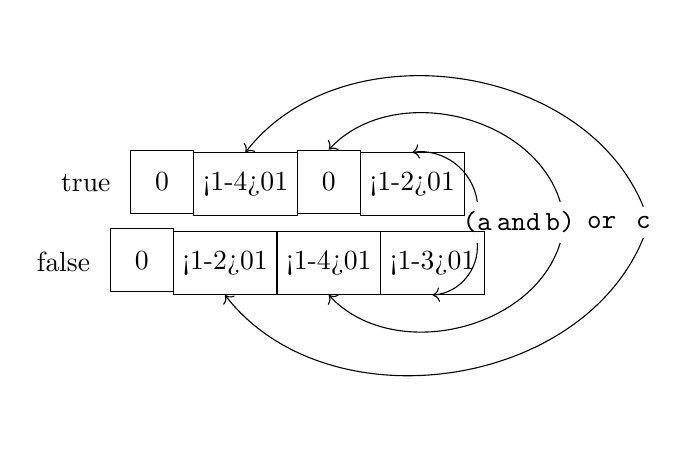
\begin{tikzpicture}
            \matrix (T) [
                matrix of nodes,
                nodes={draw, minimum size=8mm},
                column sep=-\pgflinewidth,
                label = left:true,
            ]{
                0 &
                \alt<1-4>{0}{1} &
                0 &
                \alt<1-2>{0}{1} \\
            };
            \matrix (F) [
                matrix of nodes,
                nodes={draw, minimum size=8mm},
                column sep=-\pgflinewidth,
                label = left:false,
                below of = T
            ]{
                0 &
                \alt<1-2>{0}{1} &
                \alt<1-4>{0}{1} &
                \alt<1-3>{0}{1} \\
            };

            \coordinate (anchor) at ($(T)!0.5!(F) + (+5.0em, 0.0em)$) {};
            \node (a) [node distance = 1.5em, right of=anchor] {\ttfamily (a};
            \node (1) [node distance = 1.5em, right of=a]      {\ttfamily and};
            \node (b) [node distance = 1.5em, right of=1]      {\ttfamily b)};
            \node (2) [node distance = 1.5em, right of=b]      {\ttfamily or};
            \node (c) [node distance = 1.5em, right of=2]      {\ttfamily c};

            \onslide<2->{
                \draw [->] (c.{north}) to [bend right = 60] (T-1-2.{north});
                \draw [->] (c.{south}) to [bend left  = 60] (F-1-2.{south});
                \draw [->] (b.{north}) to [bend right = 60] (T-1-3.{north});
                \draw [->] (b.{south}) to [bend left  = 60] (F-1-3.{south});
                \draw [->] (a.{north}) to [bend right = 45] (T-1-4.{north});
                \draw [->] (a.{south}) to [bend left  = 45] (F-1-4.{south});
            }
        \end{tikzpicture}

        \begin{tabular}{l}
            \visible<3->{\lstinline{f 0 0 1}} \\
            \visible<4->{\lstinline{f 0 0 0}} \\
            \visible<5->{\lstinline{f 1 0 0}} \\
        \end{tabular}
    \end{block}
\end{frame}

\begin{frame}
    \begin{block}{Local accumulators}
        \begin{align*}
            acc & \gets acc \cup B(E(u, v)) \\
            acc & \gets acc \cap M(E(u, v)) \\
        \end{align*}

        where $E(u, v)$ is the edge taken and $M(E)$ are nodes masked for $E$
    \end{block}

    \begin{block}{Remember}
        There is bijection $f: B \rightarrow \mathbb{N}$
    \end{block}
\end{frame}

\begin{frame}[fragile]
    \centering
    \lstinline{a || b}
    \begin{columns}
        \begin{column}{0.3\textwidth}
            \begin{lstlisting}[language=C, basicstyle=\small\ttfamily]
_prelude_fn:
  _t = {0}
  _f = {0}
_a:
  if (a)
    _t |= 0x01
    goto _T
  else
    _f |= 0x01
    goto _b
            \end{lstlisting}
        \end{column}

        \begin{column}{0.3\textwidth}
        \begin{lstlisting}[language=C, basicstyle=\small\ttfamily]
_b:
  if (b)
    _t &= 0x01
    _f &= 0x01
    _t |= 0x02
    goto _T
  else
    _f |= 0x02
    goto _F
        \end{lstlisting}
        \end{column}

        \begin{column}{0.3\textwidth}
            \begin{lstlisting}[language=C, basicstyle=\small\ttfamily]
_T:
  goto _E
_F:
  goto _E
_E:
  _fn_t |= _t
  _fn_f |= _f
        \end{lstlisting}
        \end{column}
    \end{columns}
\end{frame}

\begin{frame}
    \begin{columns}
        \begin{column}{0.5\textwidth}
            Local accumulators are flushed (bitwise-or) on edge-to-outcome
        \end{column}

        \begin{column}{0.5\textwidth}
            \includegraphics[
                width   = \linewidth,
                height  = 0.8\textheight,
                keepaspectratio]{graph/fig14.pdf}
        \end{column}
    \end{columns}
\end{frame}

\section{Extras}

\begin{frame}[fragile]
    \begin{columns}
        \begin{column}{0.5\textwidth}
            \centering
            \begin{lstlisting}
if (a && b && c)
    x = 1;
            \end{lstlisting}
        \end{column}

        \begin{column}{0.5\textwidth}
            \centering
            \begin{lstlisting}
if (a)
    if (b)
        if (c)
            x = 1;
            \end{lstlisting}
        \end{column}
    \end{columns}

    \centering
    \pause
    \begin{lstlisting}
    #####:    2:    if (a && b && c)
condition outcomes covered 6/6
    #####:    3:        x = 1;

    #####:    2:    if (a)
    #####:    3:        if (b)
    #####:    4:            if (c)
    #####:    5:                x = 1;
condition outcomes covered 6/6
    \end{lstlisting}
\end{frame}

\end{document}
